\documentclass{ludis}

% xelatex
\usepackage{fontspec}
\usepackage{xunicode}
\usepackage{xltxtra}

% languages
\usepackage{fixlatvian}
\usepackage{polyglossia}
\setdefaultlanguage{latvian}
\setotherlanguages{english,russian}

% bibliography
\usepackage{csquotes}
\usepackage[
    backend=biber,
    style=numeric-comp,
    natbib=true,
    url=false,
    doi=true%,
    %eprint=false
]{biblatex}
\addbibresource{bibliography.bib}

\usepackage[]{hyperref}
\hypersetup{
    colorlinks=false,
}

% toc
\setcounter{secnumdepth}{3}
\setcounter{tocdepth}{3}

%tables
\usepackage{longtable}

%papildus matemātika
\usepackage{mathtools}
\newenvironment{thmenum}
 {\begin{enumerate}[label=\upshape(\arabic*),ref=\thethm(\arabic*)]}
 {\end{enumerate}}
 
%\begin{thmenum}
%\item \label{foo} Foo
%\item \label{bar} Bar
%\item \label{baz} Baz
%\end{thmenum}

%images
\usepackage{graphicx}
\usepackage{float}

%dalīšana kolonnās
\usepackage{multicol}

%saraksti
\usepackage{enumitem}

\fakultate{Datorikas}
\nosaukums{Ultrametriski automāti}
\darbaveids{Bakalaura}
\autors{Rihards Krišlauks}
\studapl{rk09006}
\vaditajs{Prof., Dr. habil. math. Rūsiņš Mārtiņš Freivalds}
\vieta{Rīga}
\gads{2013}

\begin{document}
\maketitle

\begin{abstract-lv}
TODO
\keywords{TODO}
\end{abstract-lv}
\clearpage

\begin{abstract-en}
TODO
\keywords{TODO}
\end{abstract-en}


\tableofcontents

\specnodala{Apzīmējumu saraksts}
\setlength\LTleft{0pt}
\setlength\LTright{0pt}
\begin{longtable}{| c | p{28em} |}
  \hline
  \textbf{Apzīmējums} & \textbf{Atšifrējums}\\ 
  \endhead

  \hline
  $u_pfa$ & Galīgs (vienvirziena) $p$-ultrametrisks automāts\\
  $1u_pfa(k)$ ($2u_pfa(k)$) &  Galīgs $k$-galviņu vienvirziena (divvirzienu) $p$-ultrametrisks automāts\\
  $1U_PFA(k)$ ($2U_PFA(k)$) &  Valodu klase, ko var atpazīt ar galīgs $k$-galviņu vienvirziena (divvirzienu) $p$-ultrametrisku automātu ar amplitūdām no kādas $log$-space $p$-konstruējamas kopas\\
  $1dfa(k)$ ($2dfa(k)$) &  Galīgs $k$-galviņu vienvirziena (divvirzienu) determinēts automāts\\
  $1nfa(k)$ ($2nfa(k)$) &  Galīgs $k$-galviņu vienvirziena (divvirzienu) nedeterminēts automāts\\
  $1pfa(k)$ ($2pfa(k)$) &  Galīgs $k$-galviņu vienvirziena (divvirzienu) varbūtisks automāts\\
  $u_ptm$ &  $p$-ultrametriska Tjūringa mašīna ar $2$ lentēm, un ar $log$-space telpas sarežģītību\\
  $U_pTM$ &  Valodu klase, ko var atpazīt ar $p$-ultrametrisku Tjūringa mašīnu ar $log$-space telpas sarežģītību, un ar amplitūdām no kādas $log$-space $p$-konstruējamas kopas\\
  $\widehat{C}$ & Valodu klases $C$ apakškopa, kas satur tikai valodas formā $1^{2^n}, n \in \mathbb{N}$, jeb precīzāk -- $\widehat{C} = \left\{ h | h \in C \wedge \exists n \in \mathbb{N} : h = 1^{2^n} \right\}$\\
  \hline
\end{longtable}

\specnodala{Ievads}
Ultrametriskus automātus un Tjūringa mašīnas 2012. gadā ir ieviesis Rūsiņš Freivalds ~\citep{Freivalds2012}. Tam ir sekojuši vairāki darbi, kur dažādi to aspekti ir pētīti padziļināti. 2013. gadā Baloža un līdzautoru ~\citep{KasparsBalodis2013} darbā ir pētīta ultrametrisku automātu apraksta sarežģītība, %TODO citādāk?
tiek parādīts, ka ultrametriski automāti var sasniegt eksponenciālu pārsvaru stāvokļu skaita ziņā salīdzinot ar determinētiem automātiem, un 2013. gadā Krišlauka un līdzautoru darbā ~\citep{Krislauks2013} tiek pētīta ultrametrisku Tjūringa mašīnu galviņas pagriezienu sarežģītība.

Ultrametrisku automāti ir līdzīgi varbūtiskajiem automātiem, bet atšķirība no tiem, ultrametriskajā gadījumā netiek prasīts, lai amplitūdas, kas atbilst varbūtības jēdzienam varbūtiskajos automātos, būtu robežās no 0 līdz 1. Tie var būt patvaļīgi racionāli skaitļi. Jāpiebilst, ka Paavo Turakainen 1969. gadā ~\citep{Turakainen1969} ir ieviesis līdzīgas konstrukcijas, kur arī "varbūtības" var būt patvaļīgi lieli skaitļi, un beigu stāvokļa varbūtība tiek salīdzināta ar kādu noteiktu slieksni, turklāt ir parādīts abas konstrukcijas ir ekvivalentas. Tomēr, atšķirībā no šiem pseido-varbūtiskajiem automātiem, ultrametrisko automātu definīcijā tiek izmantots $p$-adiskās normas jēdziens.

Var teikt, ka Freivalda ieviestā definīcija ir dabīga, jo tiek pētīts vienīgais atlikušais maz pētītais nejaušību uzdošanas veids ~\citep{Freivalds2012}. Turklāt ultrametrisko automātu definīcijai ir pierādītas derīgas īpašības -- Balodis ar līdzautoriem ~\citep{KasparsBalodis2013} ir pierādījis, ka regulētu $p$-adisko automātu atpazīstamo valodu klase sakrīt ar regulāro valodu klasi.

Darbā lielākā uzmanība tiek pievērsta jautājumam par valodu hierarhiju vairākgalviņu automātu gadījumā. Determinētiem, nedeterminētiem un varbūtiskiem galīgiem automātiem ir pierādīti vairāki rezultāti gan vienvirziena gan divvirzienu automātiem ~\citep{Holzer2009,Yao1978,Monien1980,Macarie1995}. Darbā tiek pētīts vai ultrametriskiem vairākgalviņu automātiem pastāv līdzīgi rezultāti attiecībā uz valodu dalījumu hierarhijas klasēs. Kā arī tiek pētītas valodu klašu savstarpējās attiecības salīdzinot ultrametriskos automātus ar klasiskajiem.
\chapter{$p$-adiski skaitļi}
\section{Ievads $p$-adiskos skaitļos}
Par $p$-adisku ciparu sauc naturālu skaitli robežās no $0$ līdz $p-1$ (ieskaitot), kur $p$ ir patvaļīgs pirmskaitlis. Par $p$-adisku veselu skaitli sauc virkni $(a_i)_{i \in \mathbb{N}}$, kur $a_i$ ir $p$-disks cipars. To var pierakstīt kā $\cdots a_i \cdots a_2a_1a_0$.
Šī virkne atbilst naturālam skaitlim
\[\sum\limits_{i=0}^{+\infty}a_ip^i,
\]
kur $p$ ir izvēlētais pirmskaitlis un skaitīšanas sistēmas bāze. Šī virkne ir bezgalīga uz kreiso pusi. Naturālo skaitļu attēlojumiem $p$-adiskos skaitļos tikai galīgs skaits ciparu būs nenulles. Naturālam skaitlim $n$, tā $p$-adiskās reprezentācijas nenulles daļa precīzi sakritīs ar skaitļa pierakstu bāzē $p$. Kā piemēru varam apskatīt skaitli $42$ kas pie bāzes $5$ tiek pierakstīts kā $132$, un līdz ar to tā reprezentācija $5$-adiskos skaitļos ir $\cdots 0 \cdots 0132$.

Negatīviem un racionāliem skaitļiem situācija ir ievērojami citāda. Kā piemēru apskatīsim skaitli $\frac{1}{2}$ un tā $5$-adisko reprezentāciju. $\frac{1}{2}$ definē kā skaitli, ko, saskaitot ar sevi, iegūst $1$. $1$ $5$-adiskā reprezentācija ir $\cdots 0 \cdots 001$. To zinot varam izteikt $\frac{1}{2}$ $5$-adiskos skaitļos:
\[
\begin{tabular}{rrrrrrrrr|}
&$\cdots$ &2 &2 &2 &2 &2 &3\\
+&$\cdots$ &2 &2 &2 &2 &2 &3\\
\hline
\hline
&$\cdots$ &0 &0 &0 &0 &0 &1\\
\hline
\end{tabular}
\]
Interesantā kārtā gandrīz jebkuru racionālu skaitli var līdzīgi izteikt kā $p$-adisku veselu skaitli. %TODO atsauce
Izņēmumi kādam konkrētam $p$ ir skaitļi formā $\frac{a}{b}$, kur $a$ nedalās ar $p$, bet $b$ ar $p$ dalās. %TODO atsauce

Skaitļi, kas nevar tikt izteikti $p$-adiskos veselos skaitļos, var tikt attēloti $p$-adiskos (ne veselos) skaitļos. Kā piemēru varam apskatīt skaitli $\frac{1}{5}$, kuru nevar attēlot $5$-adiskos Veselos skaitļos. Tā vietā to var pierakstīt kā
\[
\cdots 0 \cdots 000,1.
\]
Jāievēro, ka arī vispārīgajā $p$-adisko skaitļu gadījumā skaitļa pieraksts ir bezgalīgs uz kreiso pusi, un galīgs uz labo.

$p$-adiskiem skaitļiem ir izpildāmas visas tās pašas aritmētiskās darbības -- saskaitīšana, atņemšana, reizināšana un dalīšana -- kas izpildāmas skaitļiem decimālajā pierakstā. Saskaitīšanu, atņemšanu un reizināšanu var izpildīt $p$-adiskos veselos skaitļos, bet dalīšanas rezultāts var būt pierakstām tikai $p$-adiskos skaitļos.

Var redzēt, ka katram racionālam skaitlim $q$ eksistē tāds pirmskaitlis $p$, ka $q$ var tikt izteikts kā $p$-adisks vesels skaitlis. To pašu nevar teikt par reāliem skaitļiem. Pastāv iracionāli skaitļi, ko nevar izteikt kā $p$-adisku skaitli nevienam $p$. Tas gan nenozīmē, ka $p$-adiski skaitļi kādam $p$ būtu reālo skaitļu apakškopa -- ir kontinuums $p$-adisku skaitļu, kas neatbilst nevienam reālam skaitlim ~\citep{Freivalds2012}.

\section{$p$-adiskas absolūtās vērtības}
Funkcija $d: X \times X \rightarrow R_{\geq 0}$, kur $X$ ir netukša kopa, tiek saukta par metriku, ja tiek apmierinātas šādas īpašības:
\begin{enumerate}
\item $d(x,y) = 0$ tad un tikai tad, ja $x = y$,
\item $d(x,y) = d(y,x)$,
\item $d(x,y) \leq d(x,z) + d(z,y)$ visiem $z \in X$.
\end{enumerate}
Metrikas funkcija tiek izmantota, lai noteiktu attālumu starp diviem kopas elementiem. Elementa attālums līdz nullei $d(x,0)$ par tā normu, vai absolūto vērtību, un tiek apzīmēts ar $||x||$.

Elementa norma apmierina šādas īpašības:
\begin{enumerate}
\item $||x||=0$ tad un tikai tad, ja $x=0$,
\item $||x*y|| = ||x||*||y||$,
\item $||x+y|| \leq ||x||+||y||$ (trīsstūra nevienādība).
\end{enumerate}
Ja trešo īpašību var aizstāt ar tas spēcīgāko variantu -- stingro trīsstūra nevienādību $||x+y|| \leq max(||x||,||y||)$ --, tad normu sauc par ultrametrisku. Citādi to sauc par Arhimedisku ~\citep{Freivalds2012}.

\begin{definicija}
Katram nenulles racionālam skaitlim $\alpha$ eksistē viennozīmīgi nosakāms sadalījums pirmreizinātājos - $\alpha = \pm 2^{\alpha_2}3^{\alpha_3}5^{\alpha_5}7^{\alpha_7} \cdots$, kur $\alpha_i$-tie ir veseli skaitļi, no kuriem tikai galīgs skaits ir nenulles. Par racionāla skaitļa $\alpha$ \textbf{$p$-adisko absolūto vērtību} (arī sauktu par \textbf{$p$-normu}) sauc 
\[
||x||_p = \begin{cases}
p^{-\alpha_p}, &\textrm{ja } \alpha \neq 0 \\
0, &\textrm{ja } \alpha = 0.
\end{cases}
\]
\end{definicija}

Ar detalizētāku izklāstu par $p$-adiskiem skaitļiem iespējams iepazīties ~\citep{Madore}.

\chapter{Vienvirziena automāti}
\section{Definīcijas}
Ultrametriski automāti tiek definēti kā Baloža un līdzautoru darbā ~\citep{KasparsBalodis2013}.
\begin{definicija}
Galīgs $p$-ultrametrisks ($U_pFA$) automāts ir kortežs $\langle S, \Sigma, s_0, \delta, F, \Lambda \rangle$, kur
\begin{itemize}
  \item $S$ ir galīga stāvokļu kopa,
  \item $\Sigma$ ir galīga kopa, ($\$ \notin \Sigma$) -- ieejas alfabēts,
  \item $s_0:S \rightarrow \mathbb{Q}_p$ ir sākotnējais amplitūdu sadalījums, %TODO vai tiešam pareizi?
  \item $\delta: \left( \Sigma \cup \left\{ \$ \right\} \right) \times S \times S \rightarrow \mathbb{Q}_p$ ir pārejas funkcija,
  \item $F \subseteq S$ ir akceptējošo stāvokļu kopa,
  \item $\Lambda = \left( \lambda, \diamond \right)$ ir akceptēšanas nosacījums, kur $\lambda \in \mathbb{R}$ ir akceptēšanas slieksnis, un $\diamond \in \left\{ \leq, \geq \right\}$.
\end{itemize}
Automāts darbojas šādi. %TODO "šādi" ir slikti
Katrā laika momentā katram automāta stāvoklim ir piekārtots $p$-adisks skaitlis, saukts par stāvokļa amplitūdu.
Automāts darbu sāk ar sākotnējo amplitūdu sadalījumu $s_0$.
Tas pa vienam pēc kārtas apstrādā ieejas vārda $w = w_1 \ldots w_n$ simbolus.
Amplitūdu sadalījums pēc $i$-tā simbola ielasīšanas tiek apzīmēts ar $s_i$, kur
$s_i(y) = \sum_{x \in S}{s_{i-1}(x) \cdot \delta \left( w_i, x, y \right) }$ katram $y \in S$.
Pēc $n$-tā simbola ielasīšanas tādā pat veidā tiek apstrādāts beigu marķieris $\$$, iegūstot beigu amplitūdu sadalījumu $s_{n+1}$.
Akceptēšanas nosacījums tiek piemērots akceptējošo stāvokļu beigu amplitūdu $p$-normu summai. Tas ir, ja $\sum_{x \in F}{\left| s_{n+1}(x) \right|_p} \diamond \lambda$, tad saka, ka vārds $w$ tiek akceptēts, citādi -- noraidīts.
\end{definicija}

Divvirzienu $k$-galviņu (kur $k\geq 1$) galīgs automāts sastāv no ieejas lentas, kas satur ieejas vārdu, pa kuru automāta galviņas drīkst pārvietoties abos virzienos, nepārkāpjot vārda galu atdalītājsimbolu  robežas. Simbolus uz ieejas lentas drīkst tikai lasīt. Formālāk:
\begin{definicija}[~\cite{Holzer2009}]
Par nedeterminētu divvirzienu $k$-galviņu galīgu automātu ($2NFA(k)$) tiek saukts kortežs $\langle S, \Sigma, k, s_0, \delta, F \rangle$, kur
\begin{itemize}
	\item $S$ ir galīga stāvokļu kopa,
	\item $\Sigma$ ir galīga kopa, ($ \triangleright,\triangleleft \notin \Sigma$) -- ieejas alfabēts,
	\item $k\geq 1$ ir galviņu skaits, 
	\item $s_0\in S$ ir sakuma stāvoklis,
	\item $\delta: \left( \Sigma \cup \left\{ \triangleright, \triangleleft \right\} \right)^k \times S \times S \rightarrow \left\{-1,0,1\right\}^k$ ir pārejas funkcija, kur $\triangleright$ un $\triangleleft$ ir vārda sākumu un beigas atdalošie simboli,
	\item $F \subseteq S$ ir akceptējošo stāvokļu kopa.
\end{itemize}
\end{definicija}
$2NFA(k)$ sākot darbu, visas tā galviņas ir novietotas uz vārda sakuma simbola. Automāts darbu beidz, kad pārejas funkcija dotajai automāta konfigurācijai nav definēta. Par $2NFA(k)$ konfigurāciju kādā laika momentā $t\geq 0$ sauc kortežu $c_t=\left(w,s,p\right)$, kur $w$ ir ieejas vārds, $s\in S$ ir pašreizējais stāvoklis, un
$p = \left( p_1, \ldots, p_k \right) \in \left\{ 0, \ldots, |w| +1 \right\}^k $
norāda pašreizējās galviņu pozīcijas. Pāreju no vienas konfigurācijas uz nākamo apzīmē ar $\vdash$. Pāreja
$\left( w, s, \left( p_1, \ldots, p_k \right) \right) \vdash \left( w, s', \left( p_1+d_1, \ldots, p_k+d_k \right) \right)$
notiek tad un tikai tad, ja
$\left(d_1, \ldots, d_k \right) \in \delta \left( \left( a_{p_1}, \ldots a_{p_k} \right) s, s' \right)$,
kur $w = a_1a_2 \ldots a_n$ ir ieejas vārds, un $a_0=\triangleright$, un $a_{n+1}=\triangleleft$. $\vdash$ refleksīvais, tranzitīvais slēgums tiek apzīmēts ar $\vdash^*$.

Valodā $L(M)$, ko akceptē automāts $M$ ietilpst tie un tikai tie vārdi, ko akceptē $M$. $2NFA(k)$ akceptē tos un tikai tos vārdus $w$, kam pastāv kāda konfigurāciju virkne, kas noved pie automāta apstāšanās akceptējoša stāvoklī, ja uz ieejas lentes ir
$\triangleright w \triangleleft$. Jeb precīzāk - 
\begin{multline*}
	L(M)=\left\{ w \in \Sigma^* | \left(w,s_0,\left(1,\ldots,1\right)\right) \vdash^* \left(w,s,\left(p_1,\ldots,p_k\right)\right), s \in F,\right.\\
	\left.\textrm{un } M \textrm{ apstājas } \left(w,s,\left(p_1,\ldots,p_k\right)\right)\right\}.
\end{multline*}
%TODO pabeigt par 2DFA(k).

\section{Attiecība pret klasiskajiem automātiem}
Vienvirziena vairākgalviņu automātiem gan determinētā gan nedeterminētā gadījumā ir pierādītas stingri iekļaujošas klases valodām, ko automāts var atpazīt atkarībā no galviņu skaita ~\citep{Holzer2009,Yao1978}. 1978. gadā ~\citet{Yao1978} parādīja, ka, lai atdalītu valodu klasi, ko var atpazīt ar $1dfa(k)$, no tās, ko var atpazīt ar $1dfa(k+1)$, pietiek ar valodu
\[
	L_n = \left\{w_1\$w_2\$ \ldots \$w_{2n} | w_i \in \left\{a,b\right\}^* \textrm{ un } w_i = w_{2n+1−i} \textrm{ visiem } 1 \leq i \leq n \right\}.
\]
Mēs apskatīsim līdzīgu valodu -- $L_k$.
\begin{teorema}
Katram $k \geq 1 \in \mathbb{N}$ eksistē valoda $L_k$, tāda ka:
\begin{enumerate}[label={(\arabic*)}]
	\item katram $k \geq 1 \in \mathbb{N}$ eksistē $1U_pFA(1)$, kas atpazīst $L_k$, %TODO varbut arī var regulētu..
	\item $L_k$ nevar atpazīt ne ar kādu $1DFA(k)$,
	\item $L_k$ nevar atpazīt ne ar kādu $1NFA(k)$.
\end{enumerate}
\end{teorema}
\begin{pieradijums} Meklētā valoda ir
\[
L_k = \left\{ w_1 1 w_2 1 \ldots 1 w_{2n} |
		w_i \in \left\{ 0 \right\}^m \wedge
		m \geq 1 \in \mathbb{N} \wedge
		w_i = w_{2n-i+1} \wedge
		n={k\choose 2}+1 \right\}.
\]
Tālāk tiks pierādīts, ka $L_k$ apmierina teorēmas punktus.

$(1)$ Tiks parādīts, kā patvaļīgai valodai $L_k$ uzbūvēt $1U_pFA(1)$ katram pirmskaitlim $p$. Automāts, sāk darbu ar amplitūdu $1$ $n$ dažādos sākuma stāvokļos $q_{1,1,1},q_{1,2,1},\ldots,q_{1,n,1}$. No katra no šiem stāvokļiem izies "zars", kas būs atbildīgs par amplitūdas krāšanu vienā no $n$ dažādiem akceptējošajiem stāvokļiem $q_{2n,1,2},q_{2n,2,2},\ldots,q_{2n,n,2}$. Katrā zarā būs divu veidu stāvokļi -- 1. grupas stāvokļi $q_{i,j,1}$ būs atbildīgi par amplitūdu "ģenerēšanu" un 2. grupas stāvokļi $q_{i,j,2}$ -- par amplitūdu "krāšanu", $i \in \left[1, 2n \right], j \in \left[1, n \right]$.

Ielasot $0$, atrodoties kādā no pirmās grupas stāvokļiem $q_{i,j,1}$, kam $i \leq n$, stāvokļa amplitūda tiek saglabāta nemainīga, un ar amplitūdu $1$ tiek pāriets uz 2. grupas stāvokli $q_{i,j,2}$, tādējādi sakrāto amplitūdu pieskaitot $q_{i,j,2}$. Ielasot $0$, 2. grupas stāvokļos $q_{i,j,2}$ amplitūda tiek saglabāta nemainīga. Ielasot $1$ 1. grupas stāvoklī $q_{i,j,1}$, kam $i < n$, automāts ar amplitūdu $j + 1$ pāriet uz stāvokli $q_{i + 1,j,1}$, tādējādi nonākot tur ar amplitūdu $(j + 1) \cdot \left| q_{i + 1,j,1} \right|$. %TODO definēt |stāvoklis|
Savukārt, ielasot $0$ 1. grupas stāvoklī $q_{i,j,1}$, kam $i > n$, stāvokļa amplitūda tiek saglabāta nemainīga, $q_{i,j,2}$ tagad tiek pāriets ar amplitūdu $-1$. Ielasot $1$ 1. grupas stāvoklī $q_{i,j,1}$, kam $i \geq n$, automāts uz stāvokli $q_{i + 1,j,1}$ pāriet ar amplitūdu $-(j + 1)$. Ielasot $1$ 2. grupas stāvoklī ar amplitūdu $1$ tiek pāriets no $q_{i,j,1}$ uz $q_{i + 1,j,1}$. Izņēmums ir stāvokļi pēdējā kolonnā -- $q_{2n,j,1}$ un $q_{2n,j,2}$ -- tā kā tie atbild par vārda pēdējā fragmenta ielasīšanu, tad tiem pāreja, ielasot $1$ netiek definēta. Automāta shēma redzama attēlā \ref{fig:1pfa}.

\begin{figure}[h!]
\centering
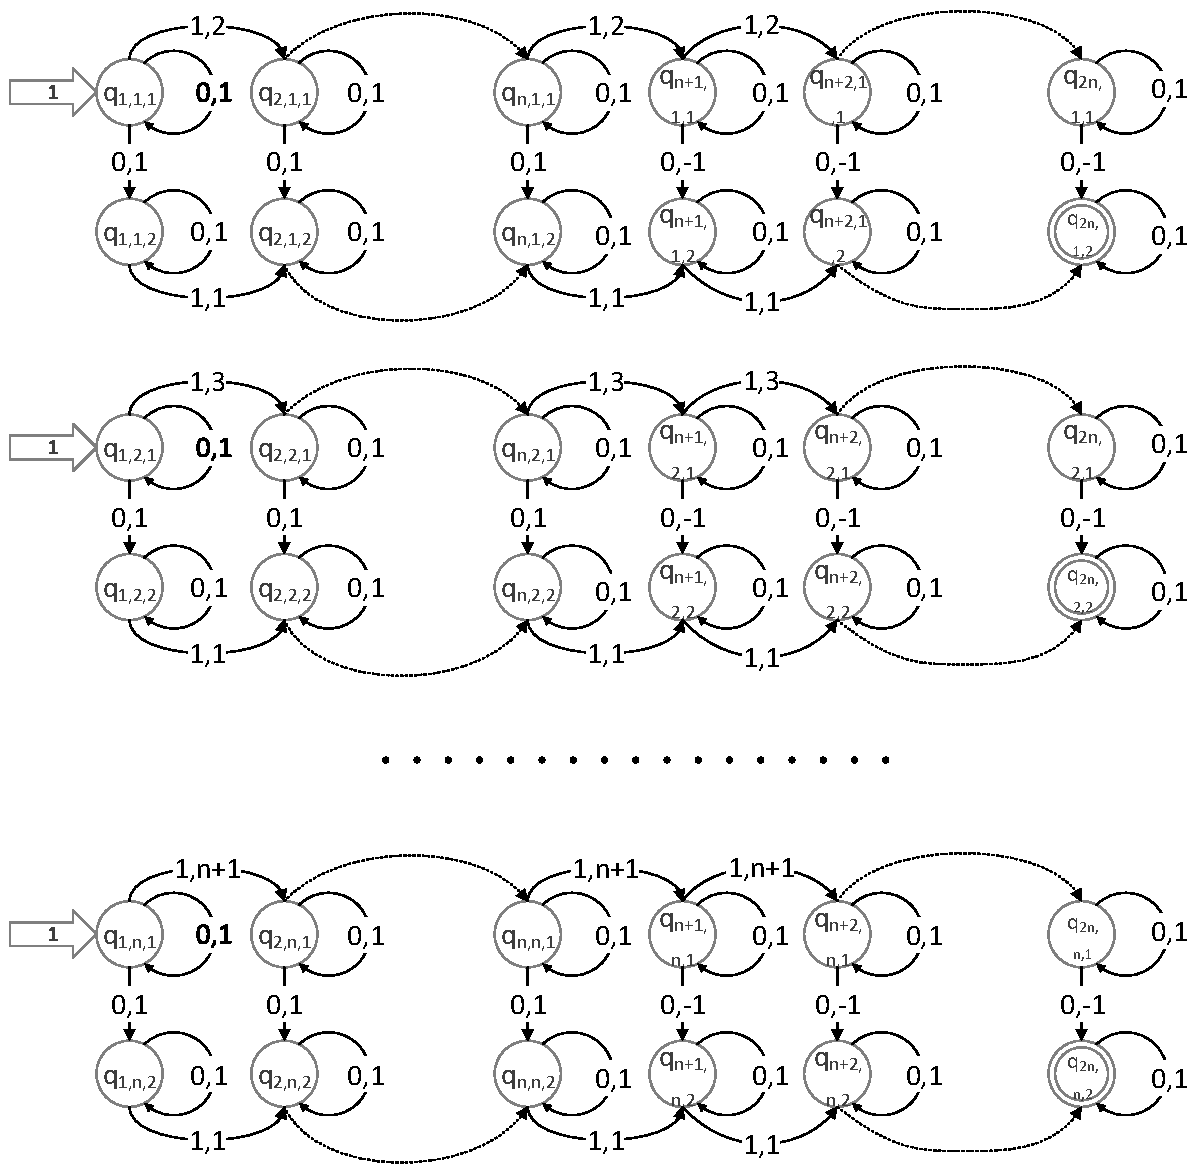
\includegraphics[width=\textwidth]{Img/1pfa.pdf}
\caption{Automāts $0^n10^m10^h1 \cdots 10^h10^m10^n$ atpazīšanai.}
\label{fig:1pfa}
\end{figure}

Rezultātā, ja tika ielasīts vārds $0^{a_1}10^{a_2}10^{a_3}1\ldots 10^{a_{2n}}$, katrā no akceptējošajiem stāvokļiem $q_{2n,j,2}$ ir sakrājusies amplitūda
\[
	a_1 + a_2 \cdot (j + 1) + a_3 \cdot (j + 1)^2 + \cdots + a_n \cdot (j + 1)^{n - 1} - a_{n+1} \cdot (j + 1)^{n - 1} - a_{n+2} \cdot (j + 1)^{n - 2} - \cdots - a_{2n},
\]
kas ir vienāda ar $0$, ja vārds pieder valodai; t.i., ja
\[
	a_1 = a_{2n} \wedge a_2 = a_{2n-1} \wedge \ldots \wedge a_n = a_{n+1}.
\]
Iegūstam, ka vārds pieder valodai tad un tikai tad, ja ir apmierināta šāda vienādojumu sistēma:
\begin{gather*}
\allowdisplaybreaks
	\begin{cases}
		a_1 + a_2 \cdot 2 + a_3 \cdot 2^2 + \cdots + a_n \cdot 2^{n - 1} - a_{n+1} \cdot 2^{n - 1} - a_{n+2} \cdot 2^{n - 2} - \cdots - a_{2n} = 0 \\
		a_1 + a_2 \cdot 3 + a_3 \cdot 3^2 + \cdots + a_n \cdot 3^{n - 1} - a_{n+1} \cdot 3^{n - 1} - a_{n+2} \cdot 3^{n - 2} - \cdots - a_{2n} = 0\\
		a_1 + a_2 \cdot 4 + a_3 \cdot 4^2 + \cdots + a_n \cdot 4^{n - 1} - a_{n+1} \cdot 4^{n - 1} - a_{n+2} \cdot 4^{n - 2} - \cdots - a_{2n} = 0\\
		\cdots \\
		\begin{split}
		a_1 + a_2 \cdot (n + 1) + a_3 \cdot (n + 1)^2 + \cdots + a_n \cdot (n + 1)^{n - 1} - a_{n+1} \cdot (n + 1)^{n - 1} \\
		\qquad- a_{n+2} \cdot (n + 1)^{n - 2} - \cdots - a_{2n} = 0\\
		\end{split}
	\end{cases}\\
\intertext{pārrakstot}
	\begin{cases}
		(a_1 - a_{2n}) + 2 \cdot (a_2 - a_{2n-1}) + 2^2 \cdot (a_3 - a_{2n-2}) + \cdots + 2^{n - 1} \cdot (a_n - a_{n+1}) = 0\\
		(a_1 - a_{2n}) + 3 \cdot (a_2 - a_{2n-1}) + 3^2 \cdot (a_3 - a_{2n-2}) + \cdots + 3^{n - 1} \cdot (a_n - a_{n+1}) = 0\\
		(a_1 - a_{2n}) + 4 \cdot (a_2 - a_{2n-1}) + 4^2 \cdot (a_3 - a_{2n-2}) + \cdots + 4^{n - 1} \cdot (a_n - a_{n+1}) = 0\\
		\cdots \\
		\begin{split}
		(a_1 - a_{2n}) + (n + 1) \cdot (a_2 - a_{2n-1}) + (n + 1)^2 \cdot (a_3 - a_{2n-2}) + \cdots \\
		\qquad+ (n + 1)^{n - 1} \cdot (a_n - a_{n+1}) = 0\\
		\end{split}	
	\end{cases}
\end{gather*}

Var redzēt, ka vienādojumu sistēmas koeficienti veido Vandermonda matricu, tātad sistēmas determinants ir nenulles, un, tā kā dotā vienādojumu sistēma ir homogēna, tai eksistē tikai triviālais atrisinājums. Tomēr ja vārds nepieder valodai var gadīties, ka kādas ne vairāk kā $4$ atsevišķas rindiņas izpildās, bet tādā gadījumā vienmēr būs vismaz viena rindiņa, kas nav vienāda ar 0 (citādi būtu nenulles risinājums, un sistēmai būtu netriviāls atrisinājums). Tātad par slieksni varam izvēlēties 0, un teikt, ka vārds pieder valodai, ja akceptējošo stāvokļu beigu amplitūdu normu summa ir $\leq 0$, un nepieder, ja citādi.

$(2)$ Pierādījis ~\citet{Freivalds1982} ~\citep{Freivalds1979}, pierādījums līdzīgai valodai atrodams arī ~\citep{Yao1978}. Pierādījuma ideja balstās uz faktu, ka divas galviņas, kas izmantotas kāda viena pāra pārbaudīšanai, nevar izmantot vairs neviena cita pāra pārbaudei. No tā arī seko, ka, ja valodas pāru fragmentu skaits $n$ ir lielāks par visu iespējamo galviņu pāru skaitu ${k\choose 2}$, tad valodu nevar atpazīt ar $k$ galviņām.

$(3)$ Pierādījis ~\citet{Freivalds1982}, pierādījums līdzīgai valodai atrodams arī ~\citep{Yao1978}.
\end{pieradijums}

Jāpiebilst, ka ar konstantu galviņu skaitu $L_k$ atpazīšanai pietiek arī varbūtiskiem automātiem. ~\citet{Freivalds1982} ir parādījis, ka jebkuram $\epsilon > 0$ eksistē $1pfa$, kas atpazīst katru vārdu $L_k$ ar varbūtību $1$, un noraida katru vārdu, kas nepieder, ar varbūtību vismaz $1 - \epsilon$.

\chapter{Divvirzienu automāti}
\section{Definīcijas}
Ultrametrisku vairākgalviņu definīcija tiek iegūta visdabiskākajā veidā paplašinot ~\citep{KasparsBalodis2013} ieviesto ultrametrisko automātu definīciju. Par pamatu tiek ņemta arī ~\citep{Holzer2009} ieviestā vairākgalviņu automātu definīcija.

\begin{definicija}
Par galīgu $k$-galviņu divvirzienu $p$-ultrametrisku automātu ($2U_pFA(k)$) tiek saukts kortežs $\langle S, \Sigma, k, s_0, \delta, F, \Lambda \rangle$, kur
\begin{itemize}
	\item $S$ ir galīga stāvokļu kopa,
	\item $\Sigma$ ir galīga kopa, ($ \triangleright,\triangleleft \notin \Sigma$) -- ieejas alfabēts,
	\item $k\geq 1$ ir galviņu skaits, 
	\item $s_0:S \rightarrow \mathbb{Q}_p$ ir sākotnējais amplitūdu sadalījums,
	\item $\delta: \left( \Sigma \cup \left\{ \triangleright, \triangleleft \right\} \right)^k \times S \times S \rightarrow \mathbb{Q}_p \times \left\{-1,0,1\right\}^k$ ir pārejas funkcija, kur $\triangleright$ un $\triangleleft$ ir vārda sākumu un beigas atdalošie simboli,
	\item $F \subseteq S$ ir akceptējošo stāvokļu kopa,
	\item $\Lambda = \left( \lambda, \diamond \right)$ ir akceptēšanas nosacījums, kur $\lambda \in \mathbb{R}$ ir akceptēšanas slieksnis, un $\diamond \in \left\{ \leq, \geq \right\}$.
\end{itemize}
\end{definicija}

$2U_pFA(k)$ darbojas līdzīgi, kā $U_pFA$, ar to izņēmumu, ka automātam tagad ir $k$ galviņas, un tās var kustēties abos virzienos līdzīgi kā $2NFA(k)$. Atšķirībā no $U_pFA$ tagad amplitūdas tiek norādītas stāvokļa un galviņu pozīcijas pārim. Amplitūda ar kādu automāts atrodas stāvoklī $y \in S$ ar galviņām pozīcijās
$\left( p_1, \ldots, p_k \right) \in \left\{ 0, \ldots, |w| +1 \right\}^k $
pēc $i$-tās darbības veikšanas tiek apzīmēta ar
\[
s_i (y, (p_1, \ldots, p_k)) =
\sum_{\mathclap{\substack{ x \in S \wedge \\
		\exists (p'_1, \ldots, p'_k):
		(p'_1, \ldots, p'_k) +
		\delta ((w_{p'_1}, \ldots, w_{p'_k}), x, y)_2 =
		(p_1, \ldots, p_k)}}}
	{s_{i-1}(x) \cdot \delta ((w_{p'_1}, \ldots, w_{p'_k}), x, y)_1 }
\].

Līdzīgi kā iepriekš, automātam beidzot darbu, akceptēšanas nosacījums tiek piemērots akceptējošo stāvokļu beigu beigu amplitūdu $p$-normu summai. Tas ir, ja
\[
\sum_{\mathclap{\substack{x \in F \wedge\\
		\exists (p_1, \ldots, p_k):
		\textrm{ automāts beidz darbu stāvoklī } x
		\textrm{ ar galviņām pozicijās } (p_1, \ldots, p_k) }}}
	{\left| s_{n+1}(x, (p_1, \ldots, p_k)) \right|_p} \diamond \lambda
\]
, tad saka, ka vārds $w$ tiek akceptēts, citādi -- noraidīts.

%TODO sameklēt visas pareizrakstības kļūdas, piem., ari

Ultrametriskas Tjūringa mašīnas darbā tiks izmantotas, lai pierādītu rezultātus vairākgalviņu automātu sadalījumam hierarhijas klasēs.

Ultrametriskas Tjūringa mašīnas definīcija tiek iegūta dabiskā veida paplašinot J. Hopcroft un J. Ullman ~\citep{Hopcroft1979} 1979. gadā ieviesto definīciju. Ērtības labad definēsim mašīnu ar vairākām darba lentēm.
\begin{definicija}
Par $p$-ultrametrisku Tjūringa mašīnu ar $k$ darba lentēm $(U_pTM(k))$ sauc kortežu $M= \langle Q, \Gamma, b, \Sigma, \delta, q_0, F \rangle$, kur:
\begin{itemize}
	\item $Q$ ir galīga netukša stāvokļu kopa,
	\item $\Gamma$ ir galīga netukša kopa -- darba alfabēts,
	\item $b \in \Sigma$ ir "tukšais" simbols (drīkst atrasties uz lentes neierobežoti daudz eksemplāros),
	\item $\Sigma\subseteq\Sigma\setminus\{b\}$ ieejas alfabēts,
	\item $q_0 \in Q_p$ ir sākotnējais amplitūdu sadalījums,
	\item $F \subseteq Q$ ir akceptējošo stāvokļu kopa.
	\item $\delta: Q \setminus F \times \Sigma^k \rightarrow Q \times \left(\Sigma \times \{L,N,R\} \times \mathbb{Q}_p \right)^k$ ir daļēji definēta pārejas funkcija, kur $L$ apzīmē mašīnas galviņas pabīdīšanu pa kreisi , $R$ -- pabīdīšanu pa labi, un $N$ norāda, ka mašīnas galviņa netiek pārvietota, un $\mathbb{Q}_p$ ir amplitūda, ar kādu tiek veikta pāreja.
\end{itemize}
\end{definicija}

Līdzīgi kā ultrametrisku vairākgalviņu automātu gadījumā mašīna ar noteiktu amplitūdu atrodas kāda no tās iespējamajām konfigurācijām, bet tagad konfigurācija iekļauj vadības bloka stāvokli un visu $k$ lenšu saturu. Amplitūda, ar kādu mašīna $i$-tajā solī atrodas kāda konfigurācijā tiek aprēķināta analogi tam, kā norādīts ultrametrisko vairākgalviņu automātu gadījumā.
%TODO ko nozīmē, ka mašīna akceptē vārdu

Ultrametriski vairāku skaitītāju automāti arī tiks izmantoti kā starpposms pierādījumos.
\begin{definicija}
Galīgs $p$-ultrametrisks $k$ reģistru automāts (turpmāk arī mašīna) ($2U_pRA(k)$) sastāv no vadības bloka ar ultrametriskām pārejām, un $k$ reģistriem, kas satur naturālus skaitļus. Automāts sak darbu ar ieejas vārdu pirmajā reģistrā, un ar amplitūdu, kas atbilst sākotnējajam emplitūdu sadalījumam, kāda no vadības bloka stāvokļiem. Katram no reģistriem var tikt pielietots predikāts $\stackrel{?}{=} 0$ un operācija $+1$ vai $-1$. Katrai vadības bloka pārejai var tikt norādīts predikāts vai operācija, kas izpildās veicot pāreju, kā arī amplitūda. Vārda akceptēšanas kritēriji ir analogi ultrametrisko automātu definīcijā izmantotajiem.
\end{definicija}

\section{Ultrametriska automāta simulācija}
Nākamās nodaļas pierādījumos tiks izmantota iespēja ultrametrisku vairākgalviņu automātu simulēt ar ultrametrisku Tjūringa mašīnu. Šeit tiks parādīti vispārīgie principi, kas ir šādas simulācijas pamatā, izmantotās idejas ir līdzīgas kā ~\citep{Macarie1995} varbūtisko automātu gadījumā.

Vienkāršības labad var pieņemt, ka simulējamajam automātam no katra stāvokļa iziet ne vairāk kā $2$ pārejas. Tiks aprakstīts veids, kā veidot $p$-ultrametrisku $2$ lenšu Tjūringa mašīnu, kas, ieejā saņemot $p$-ultrametriska $k$ galviņu automāta aprakstu, akceptē tos un tikai tos vārdus, ko simulējamais automāts. Tā kā turpmākajā darbā šādas simulācijas nepieciešamība tiks apskatīta tikai darbojoties ar vārdiem viena burta alfabētā, tad tiks parādīts veids, kā automāta aprakstu uzdot izmantojot viena burta alfabētu; konkrētāk -- vārdus formā $1^{2^n}, n \in \mathbb{N}$. Vēl tiek prasīts, lai simulējamā automāta amplitūdas būtu $log$-space $p$-konstruējamas skaitļu kopas. Par $log$-space $p$-konstruējamu skaitļu kopu sauksim tādu kopu, kam eksistē $p$-ultrametriska Tjūringa mašīna ar $log$-space telpas sarežģītību, kas, saņemot ieejā kaut kādu skaitļa, kas pieder kopai, "aprakstu", spēj nonākt kādā īpaši atzīmētā stāvoklī ar amplitūdu kas atbilst "aprakstam". Zemāk tiks parādīts, ka šāda ultrametriska Tjūringa mašīna pastāv amplitūdām racionālos skaitļos binārajā pierakstā.
%TODO pateikt, kāpēc vajag log space telpas sarežģītību

$p$-Ultrametriska galīga $k$ galviņu automāta aprakstu var uzdot ar bināru virkni, pēc kārtas norādot:
\begin{itemize}
	\item automāta stāvokļu skaitu,
	\item galviņu skaitu,
	\item pārejas starp stāvokļiem un to amplitūdas %TODO cik daudz vietas aizņem?
\end{itemize}

Simulācija tiek realizēta šādi. $p$-Ultrametriska galīga $k$ galviņu automāta ar pāreju amplitūdām no $log$-space $p$-konstruējamas kopas, saukta par $A$, simulēšanai tiek veidota $p$-ultrametriska $2$ lenšu Tjūringa mašīna, saukta par $T$. $T$ uz ieejas lentes tiek padots $A$ apraksts viena burta alfabētā formā $1^{2^n}, n \in \mathbb{N}$. Sākot darbu $T$ ielasa ieejas vārdu un determinēti, pārejas veicot ar amplitūdu $1$, sagatavo 2. lentu, tur ierakstot skaitli $n$ binārā pierakstā. $n$ ir simulējamā automāta $A$ apraksts. Tiek arī izdalīta vieta apjomā $k \cdot n$ $k$ skaitītājiem, kas norādīs $A$ galviņu pozīcijas. Tālākajā simulācijas gaitā tiks izmantota tikai 2. lente (lai arī rakstīšanai var izmantot abas lentes, ērtībai sauksim 2. lenti par darba lenti).

Atceramies, ka $A$ savas darbības laikā iziet cauri vairāku konfigurāciju virknei, un katrā laika momentā $A$ var "paralēli" būt vairākās konfigurācijās ar dažādām amplitūdām. %TODO pateikt šo pie definīcijas
Ja $A$ atrodas kāda konfigurācijā ar amplitūdu $a$, tad $T$ to simulēs, ar atbilstošo amplitūdu atrodoties konfigurācijā, kur darba lentes saturs atbilst attiecīgajai $A$ konfigurācijai.

Lai parādītu, ka $T$ var šādā veidā simulēt $A$, jāparāda, ka $T$ ir spējīgs veikt katru $A$ pāreju. Parādīsim, ka, ja $A$ ir pāreja no $q_1$ uz $q_2$ ar amplitūdu $a_1$ (pieņemsim, ka tā ir apzīmēta ar numuru $i$ ) un pāreja no $q_1$ uz $q_3$ ar amplitūdu $a_2$ (pieņemsim, ka tā ir apzīmēta ar numuru $j$), tad $T$ atrodoties $q_1$ atbilstošajā konfigurācijā var "paralēli" veikt pārejas uz $q_2$ un $q_3$ atbilstošajām konfigurācijām ar attiecīgajām amplitūdām. Tas tiek darīts, $U$ sazarojoties un abos gadījumos ar amplitūdu $1$ īpašā vietā uz lentes ierakstot vai nu skaitli $i$ vai $j$, kas attiecīgi atbilst pirmajai un otrajai $A$ pārejai. Ierakstīšana tiek veikta determinēti, pārejas veicot ar amplitūdu $1$. Tālāk tiek darbināta apakšprogramma, kas ierakstītajam skaitlim atbilstošo amplitūdu $a_1$ vai $a_2$ ielasa īpašā stāvoklī $q_u$ (tā kā tika uzstādīta prasība, ka ir no $log$-space $p$-konstruējamas kopas, tad šāda apakšprogramma eksistē). Tālāk no stāvokļa $q_u$ tiek pāriets uz bloku, kas darba lenti izmaina atbilstoši pārejai, kas atbilst uz lentas ierakstītajam skaitlim (tas tiek darīts determinēti, pārejas veicot ar amplitūdu $1$). Tā kā vienīgā pāreja, kas ir atšķirīga no $1$ tiek veikta, pārejot no $q_u$, tad darbības beigās uz $U$ darba lentes ar amplitūdu $1 \cdot 1 \cdots 1 \cdot a_1 = a_1$ ir ieraksts, kas atbilst $A$ konfigurācijai pēc pārejas $i$ izdarīšanas, un ar amplitūdu $1 \cdot 1 \cdots 1 \cdot a_2 = a_2$ -- ieraksts, kas atbilst $A$ konfigurācijai pēc pārejas $j$ izdarīšanas.

%TODO zimējums

\begin{teorema}
Racionālie skaitļi veido $log$-space $p$-konstruējamu kopu.
\end{teorema}
\begin{pieradijums}
Parādīsim, ka jebkuram pirmskaitlim $p$ eksistē $p$-ultrametriska vienas lentes Tjūringa mašīna, kas ieejā saņemot racionāla skaitļa $a$ pierakstu binārā formā, savas darbības beigās nonāk īpašā stāvoklī $q_u$ ar amplitūdu $a$.

Skaitlis $a$ uz lentes tiks padots formā
\[
	\triangleright a_n a_{n-1} \cdots a_1 \cdot a_0 | a_{-1} a_{-2} \cdots a_{-m} \triangleleft,
\]
kur $\sum\limits_{i=-m}^n a_i \cdot 2^i = a$ ($|$ ir atdalītājsimbols). Mašīna sākotnēji, ignorējot atdalītājsimbolu, cikliski no skaitļa $a \cdot 2^m$ atņem $1$, katru reizi to izdarot, palielinot $q_u$ amplitūdu par $1$. Kad uz lentas atrodas vairs tikai
\[
	00 \cdots 0|00 \cdots 0,
\]
mašīna $q_u$ sakrāto amplitūdu izdala ar $2^m$. $\rightarrow_i$ norāda, ka pāreja tiek veikta ar amplitūdu $i$.

Tjūringa mašīnas programmas teksts.
\begin{multicols}{2}
	\begin{align*}
	\allowdisplaybreaks
	\shortintertext{Atņem $1$ no $a$}
		q_0\triangleleft & \rightarrow_1 q_1\triangleleft L\\
		q_10 & \rightarrow_1 q_11L\\
		q_11 & \rightarrow_1 q_20R\\
		q_1| & \rightarrow_1 q_1|L\\
	\shortintertext{Iet atpakaļ uz $a$ sākumu}
		q_20 & \rightarrow_1 q_20R\\
		q_21 & \rightarrow_1 q_21R\\
		q_2| & \rightarrow_1 q_2|R\\
		q_2\triangleleft & \rightarrow_1 q_1\triangleleft L\\
	\shortintertext{Palielina īpašā stavokļa apmlitūdu par $1$}
		q_2\triangleleft & \rightarrow_1 q_u'\triangleleft L\\
	\shortintertext{Atrodas $a$ sakumā, jo tas jau ir $0$}
		q_1\triangleright & \rightarrow_1 q_3\triangleright R\\
	\shortintertext{Nodzēš pēdejā gajienā kļūdaini sarakstīto}
		q_30 & \rightarrow_1 q_30R\\
		q_31 & \rightarrow_1 q_31R\\
		q_3| & \rightarrow_1 q_3|R\\
	\shortintertext{Dala īpašā stāvokļa amplitūdu, atbilstoši ciparu skaitam aiz komata}
		q_3\triangleleft & \rightarrow_1 q_u'\triangleleft L\\
		q_u'0 & \rightarrow_\frac{1}{2} q_u'0L\\
		q_u'1 & \rightarrow_\frac{1}{2} q_u'1L\\
	\shortintertext{Iet uz $a$ sākumu}
		q_u'| & \rightarrow_1 q_u|R\\
		q_u0 & \rightarrow_1 q_u0R\\
		q_u1 & \rightarrow_1 q_u1R\\
	\end{align*}
\end{multicols}
\end{pieradijums}
%TODO pateikt, ka nav atkarīgs no p

\section{Vairākgalviņu automāti}
~\citet{Monien1980} ir parādījis, ka galīgiem determinētiem un nedeterminētiem automātiem valodu klase, ko var atpazīt, izmantojot $k$ galviņas, stingri iekļaujas valodu klasē, ko var atpazīt ar $k+1$ galviņu. Vēlāk, izmantojot līdzīgas metodes, ~\citet{Macarie1995} pierādīja atbilstošos rezultātus arī galīgiem varbūtiskiem automātiem. Tālāk tiks pierādīts, ka tādi paši rezultāti ir spēkā arī ultrametriskiem automātiem.

\begin{teorema} \label{atdalisana}
Katram naturālam skaitlim $k$ un pirmskaitlim $p$ izpildās
\[
	\widehat{U_pFA(k)} \subsetneqq \widehat{U_pTM}.
\]
\end{teorema}
\begin{pieradijums}
Veidosim īpašu $p$-ultrametrisku Tjūringa mašīnu ar $2$ lentēm, un ar $log$-space telpas sarežģītību, sauktu par $T$, un parādīsim, ka tās atpazītā valoda nevar tikt atpazīta ar nevienu $p$-ultrametrisku automātu ar $k$ galviņām (visiem $k$).

Līdzīgi kā parādīts nodaļas sākumā, $T$ veidosim tā, ka tā simulē ieejā saņemtu $u_pfa(k)$, sauktu par $A$. Atšķirībā no apraksta, $A$ "aprakstā" tieša veidā netiek iekļauts ieejas vārds, ko $A$ apstrādā. Tā vietā $A$ tiks darbināts uz ieejas virknes, t.i. -- uz sava "apraksta".

Precīzāk -- $T$ uz 1. lentes atrodas vārds $1^m, m \in \mathbb{N}$, $T$ pārbauda, vai tas ir formā $1^{2^n}, n \in \mathbb{N}$ (vārdu noraida, ja tas neatbilst) un uz 2. lentes (sauksim par darba lenti) uzraksta $n$ binārā pierakstā, aizņemot $log(n)$ vietas. Tiek pārbaudīts, vai $n$ pieraksts sintaktiski atbilst kādam $u_pfa(k)$; vārdu noraida, ja tas neatbilst. Tālāk $T$ uz darba lentes tiek izdalīta vieta $k$ skaitītājiem, kas norādīs $A$ galviņu pozīcijas uz ieejas vārda. Tā kā kā vērtības var būt robežās $\left[0, \ldots, 1^{2^n} \right]$, tad tam tiek patērēts $k \cdot log(2^n)= k \cdot n$ vietas. %TODO nevajag novērtēt visur ar O()?
Tas tiek darīts determinēti, pārejas veicot ar amplitūdu $1$. Tālāk $T$ darbina uz ieejas virknes kā parādīts nodaļas sākumā (1. lentes galviņa vairs netiek kustināta, tiek pārbaudīts, vai galviņām atbilstošie skaitītāji ir vārda robežās, vai nē). Rezultātā $T$ ar attiecīgajām amplitūdām ir nonācis visās iespējamajās konfigurācijās, kur $A$ var nonākt apstrādājot vārdu. Tālāk $T$ skatās, vai darba lentes saturs liecina, ka $A$ ir nonācis akceptējošā stāvoklī, un vārdu noraida, ja $A$ ir akceptējošā stāvoklī, un akceptē, ja $A$ nav nonācis akceptējoša stāvoklī. Tādējādi $T$ ar tādu pašu amplitūdu kā $A$, dod pretēju rezultātu.

Apskatīsim valodu $L(T)$, ko akceptē $T$. Ir skaidri redzams, ka katram $u_pfa(k)$, ko apzīmēsim ar $J$, eksistē tāds vārds, kas pieder $L(T)$, bet nepieder $L(J)$, vai nepieder $L(T)$, bet pieder $L(J)$ -- $J$ apraksts.
\end{pieradijums}

Tāpat kā ~\citep{Macarie1995} un ~\citep{Monien1980} tiks izmantota funkcija
\[
	f_k : \left\{ 1^{2^n} | n \in \mathbb{N} \right\} \rightarrow \left\{ 1^{2^n} | n \in \mathbb{N} \right\} \textrm{, kur } f_k( 1^{2^n}) = 1^{2^{k \cdot n}}
\]

\begin{lemma} \label{skaititaji}
Katrai valodai $L \in \widehat{U_pTM}$ eksistē naturāls skaitlis $u$, tāds ka
\[
	f_u(L) \in \widehat{U_pFA(5)}.
\]
\end{lemma}
\begin{pieradijums}
Parādīsim, kā $u_ptm$, sauktu par $T$, kas atpazīst $L$, pārveidot par citu $u_ptm$, sauktu par $T'$, ko iespējams aizstāt ar $p$-ultrametrisku $3$ skaitītāju mašīnu, no kā viegli seko, ka eksistē $u_pfa(k)$, kas atpazīst ar $f_u$ "izstiepto" $L$ variantu.

Veidosim $T'$, kas simulēt $T$. $T'$ uz darba lentes glabās šādu informāciju:
\begin{itemize}
	\item ieejas vārda bināru reprezentāciju,
	\item $T$ 1. lentes galviņas pozīciju (sauksim par ieejas lenti),
	\item $T$ 2. lentes saturu (sauksim par darba lenti), %kas aizņem $O(log n)$ vietu,
	\item $T$ darba lentes galviņas pozīciju.
\end{itemize} %TODO telpas novērtējumi
Uz $T'$ darba lentes $T$ simulēšanu veikt ir vienkāršāk nekā ultrametrisko automātu gadījumā, jo $T'$ var izmantot oriģinālo $T$ vadības bloku, un pārejas nav jāsimulē uz lentes. $T$ simulācijā $T'$ izmanto tikai darba lenti.

Var redzēt, ka var uzbūvēt $T'$ atbilstošu $p$-ultrametrisku $3$ reģistru mašīnu. Ja ieejas vārds ir $1^{2n}$, tad mašīna sak darbu ar $n$ bināro reprezentāciju pirmajā reģistrā un ar $0$ pārējos. Var pārliecināties, ka izmantojot pirmos divus reģistrus, kuros darbības laikā atrodas skaitļi $v$ un $h^{rev}$, un trešo reģistru kā palīgmainīgo, iespējams simulēt $T'$ darba lenti. Lai to panāktu tiek izmantota iespēja reģistriem pieskaitīt un atņemt $1$, un tos saturu reizināt un dalīt ar $2$, ko palīdz realizēt trešais -- papildus reģistrs. Tas shematiski parādīts attēlā \ref{fig:skaititaji}.

\begin{figure}[h!]
\centering
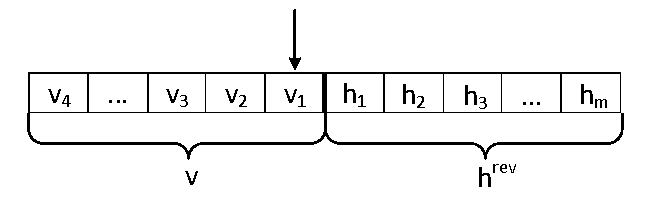
\includegraphics[width=0.8\textwidth]{Img/skaititaji.pdf}
\caption{Tjūringa mašīnas lentes satura simulēšana ar reģistriem.}
\label{fig:skaititaji}
\end{figure}

Tā kā vairākgalviņu automāta galviņas pozīcija tiešā veidā atbilst skaitlim skaitītajā. Tad $5$ skaitītāju mašīnu var aizstāt ar $p$-ultrametrisku galīgu $5$ galviņu automātu. Tomēr, tā kā vairākgalviņu automāta galviņas nedrīkst iziet ārpus lentes robežām, tad tas nevar simulēt patvaļīgi lielus skaitītājus. To, ka ieejas vārdi ir pietiekami gari, lai automāts simulētu $T'$ darba lentes saturu, nodrošina piemeklējot pietiekami lielu $u$.
\end{pieradijums}
%TODO definēt skaitītaju mašīnu
%TODO deterministiski -> determinēti

\begin{lemma} \label{reizinajums}
Visām valodām $L \in \widehat{U_pTM}$ un visiem $u, v \geq 1, u, v \in \mathbb{N}$ izpildās
\[
	f_u(L) \in \widehat{U_pFA(v)} \Rightarrow L \in \widehat{U_pFA(u \cdot v)}.
\]
\end{lemma}
\begin{pieradijums}
Premisā minēto $U_pFA(v)$ sauksim par $A$, un sekās minēto $U_pFA(u \cdot v)$ -- par $A'$. %TODO premisa, sekas - varbūt nevajag
Apskatīsim $A$ darbību, ja ieejā saņemts vārds $f_u(l), l = 1^{2^n} \in L, n \in \mathbb{N}$. Pozīciju uz ieejas vārda katrai no automāta $A$ $v$ galviņām var aprakstīt naturālu ar skaitli robežās $\left[0, 2^{u \cdot n} -1 \right]$. Šo skaitli var arī izteikt ar $u$ cipariem pie bāzes $2^n$. Tā kā katras $A'$ galviņas pozīciju uz ieejas vārda varam aprakstīt ar ciparu pie bāzes $2^n$, tad katru no $A$ galviņām var simulēt ar $u$ $A'$ galviņām. Tā kā katrai $A$ galviņas kustībai atbilst kāda $A'$ galviņas kustība, tad atbilstošās pārejas var veikt ar vienādām amplitūdām, un vārdu akceptēšanas amplitūdas saglabājas.

Šī simulācija notiek līdzīgi kā varbūtiskajā gadījumā ~\citep{Macarie1995}. %TODO pārbaudīt vai nav arī nedeterminētajā
\end{pieradijums}

\begin{lemma} \label{plus1}
Visām valodām $L \in \widehat{U_pTM}$ un visiem $u > v > 1, u, v \in \mathbb{N}$ izpildās
\[
	f_{u+1}(L) \in \widehat{U_pFA(v)} \Rightarrow f_u(L) \in \widehat{U_FA(v + 1)}.
\]
\end{lemma}
\begin{pieradijums}
Premisā minēto $U_pFA(v)$ sauksim par $A$, un sekās minēto $U_pFA(v + 1)$ -- par $A'$. %TODO premisa, sekas - varbūt nevajag
Apskatīsim $A$ darbību, ja ieejā saņemts vārds $f_{u+1}(l), l = 1^{2^n} \in L, n \in \mathbb{N}$. Pozīciju uz lentes katrai no automāta $A$ $v$ galviņām var aprakstīt naturālu ar skaitli $h_i$ robežās $h_i \in \left[0, 2^{(u + 1) \cdot n} + 1 \right]$. Simulēsim $h_i$ pozīciju automātā $A'$ ar galviņu $g_i$ un papildus skaitli $x_i \in \left[ 0, 2^n \right]$, tā, ka $h_i = g_i + x_i \cdot 2^{u \cdot n}$. Var redzēt, ka šādi var aprakstīt skaitļus vajadzīgajā intervālā
\begin{align*}
	2^{u \cdot n} + (2^n - 1) \cdot 2^{u \cdot n} & =\\
	2^{u \cdot n} \cdot (1 + (2^n - 1)) & =\\
	2^{u \cdot n + n} & =\\
	2^{(u + 1) \cdot n}.\\
\end{align*}
Visi skaitā $v$ nepieciešamie $x_i$ tiek kodēti ar $A'$ $(v+1)$-mo galviņu. %TODO pateikt, ka tas nav triviāli?
To var panākt, ja uz $A'$ lentes ir pietiekami daudz vietas, t.i., ja $(2^n)^v < 2^{u \cdot n}$, no kā seko prasība $v < u$.

Tā kā katrai $A$ galviņas kustībai atbilst kāda $A'$ galviņas kustība, tad atbilstošās pārejas var veikt ar vienādām amplitūdām, un vārdu akceptēšanas amplitūdas saglabājas.

Šīs simulācija notiek līdzīgi kā varbūtiskajā ~\citep{Macarie1995} un nedeterminētajā ~\citep{Monien1980} gadījumā.
\end{pieradijums}

Rezultāts par $k + 1$ galviņas pārākumu pār $k$ viegli seko no iepriekšējām lemmām un teorēmas \ref{atdalisana}.
\begin{teorema}
Visiem $k \geq 2 \in \mathbb{N}$ izpildās
\[
	\widehat{U_pFA(k)} \subsetneqq \widehat{U_pFA(k + 1)}.
\]
\end{teorema}
\begin{pieradijums}
Pierādām no pretējā, parādot, ka no pieņēmuma, ka eksistē tāds $h \geq 2$, kam $\widehat{U_pFA(h)} = \widehat{U_pFA(h + 1)}$ seko, $\widehat{U_pFA(h \cdot (h + 1))} = \widehat{U_pTM}$, kas ir pretrunā ar teorēmu \ref{atdalisana}.

Ņemam kādu $L \in \widehat{U_pTM}$ kādam pirmskaitlim $p$. No lemmas \ref{skaititaji} seko, ka eksistē tāds $m \in \mathbb{N}$, ka $f_m(L) \in \widehat{U_pFA(5)}$. Tātad arī $f_m(L) \in \widehat{U_pFA(h)}$. No lemmas \ref{plus1} seko, ka, ja $m > h + 1$ tad $f_{m-1}(L) \in \widehat{U_pFA(h + 1)} = \widehat{U_pFA(h)}$. Ņemam $m = m - 1$, un atkārtojam, līdz nonākam pie $f_m(L) \in \widehat{U_pFA(h)}$, un $m = h + 1$. Tad no lemmas \ref{reizinajums} seko, ka, ja $f_m(L) \in \widehat{U_pFA(h)}$, tad $L \in \widehat{U_pFA(h \cdot m)} = \widehat{U_pFA(h \cdot (h + 1))}$. Kas ir pretrunā ar teorēmu \ref{atdalisana}.
\end{pieradijums}
\begin{sekas}
Tā kā $U_pFA(k + 1)$ sevī iekļauj $U_pFA(k)$, un tikko tika parādīts, ka eksistē tāda valoda, ko var atpazīt ar $k+1$ galviņu, bet nevar ar $k$, tad galviņu hierarhijas rezultāts ir spēkā arī valodām vairāku burtu alfabētā:
\[
	U_pFA(k) \subsetneqq U_pFA(k + 1).
\]
\end{sekas}

\chapter{Secinājumi}
TODO

\printbibliography

\end{document}